\clearpage
\cleardoublepage

\chapter{Introduction}

Different Fields of science deal with geospatial data regularly for analysis.
The most prominent use of geospatial data in the atmospheric sciences. Some of the fields
which heavily depend on the geospatial data are Climatology, Oceanography, and Meteorology.

In the field of Meteorology, weather forecasting is an essential task. Which is done using complex statistical models and complex computations.
These complex computations are due to the geospatial data's
complexity and volume.

Given the complex nature of geospatial data,
Deep Neural Networks emerge as the most suitable contender for the analysis thereof. Convolutional Neural Networks (CNNs) have demonstrated advancements in the field of computer
vision. Convolutional Neural Networks (CNNs) are now employed to analyze geospatial data. The CNNs can process the data consisting of multiple channels, as they process
data in the images containing RBG channels. This feature is also compatible with the geospatial data layered in nature and contains different geographical properties in its layers
(channels).

Work which is being done on the geospatial data is concentrated on specific regions of the globe.
\begin{figure}[h]
    \centering
    \begin{minipage}{0.45\textwidth}
        \centering
        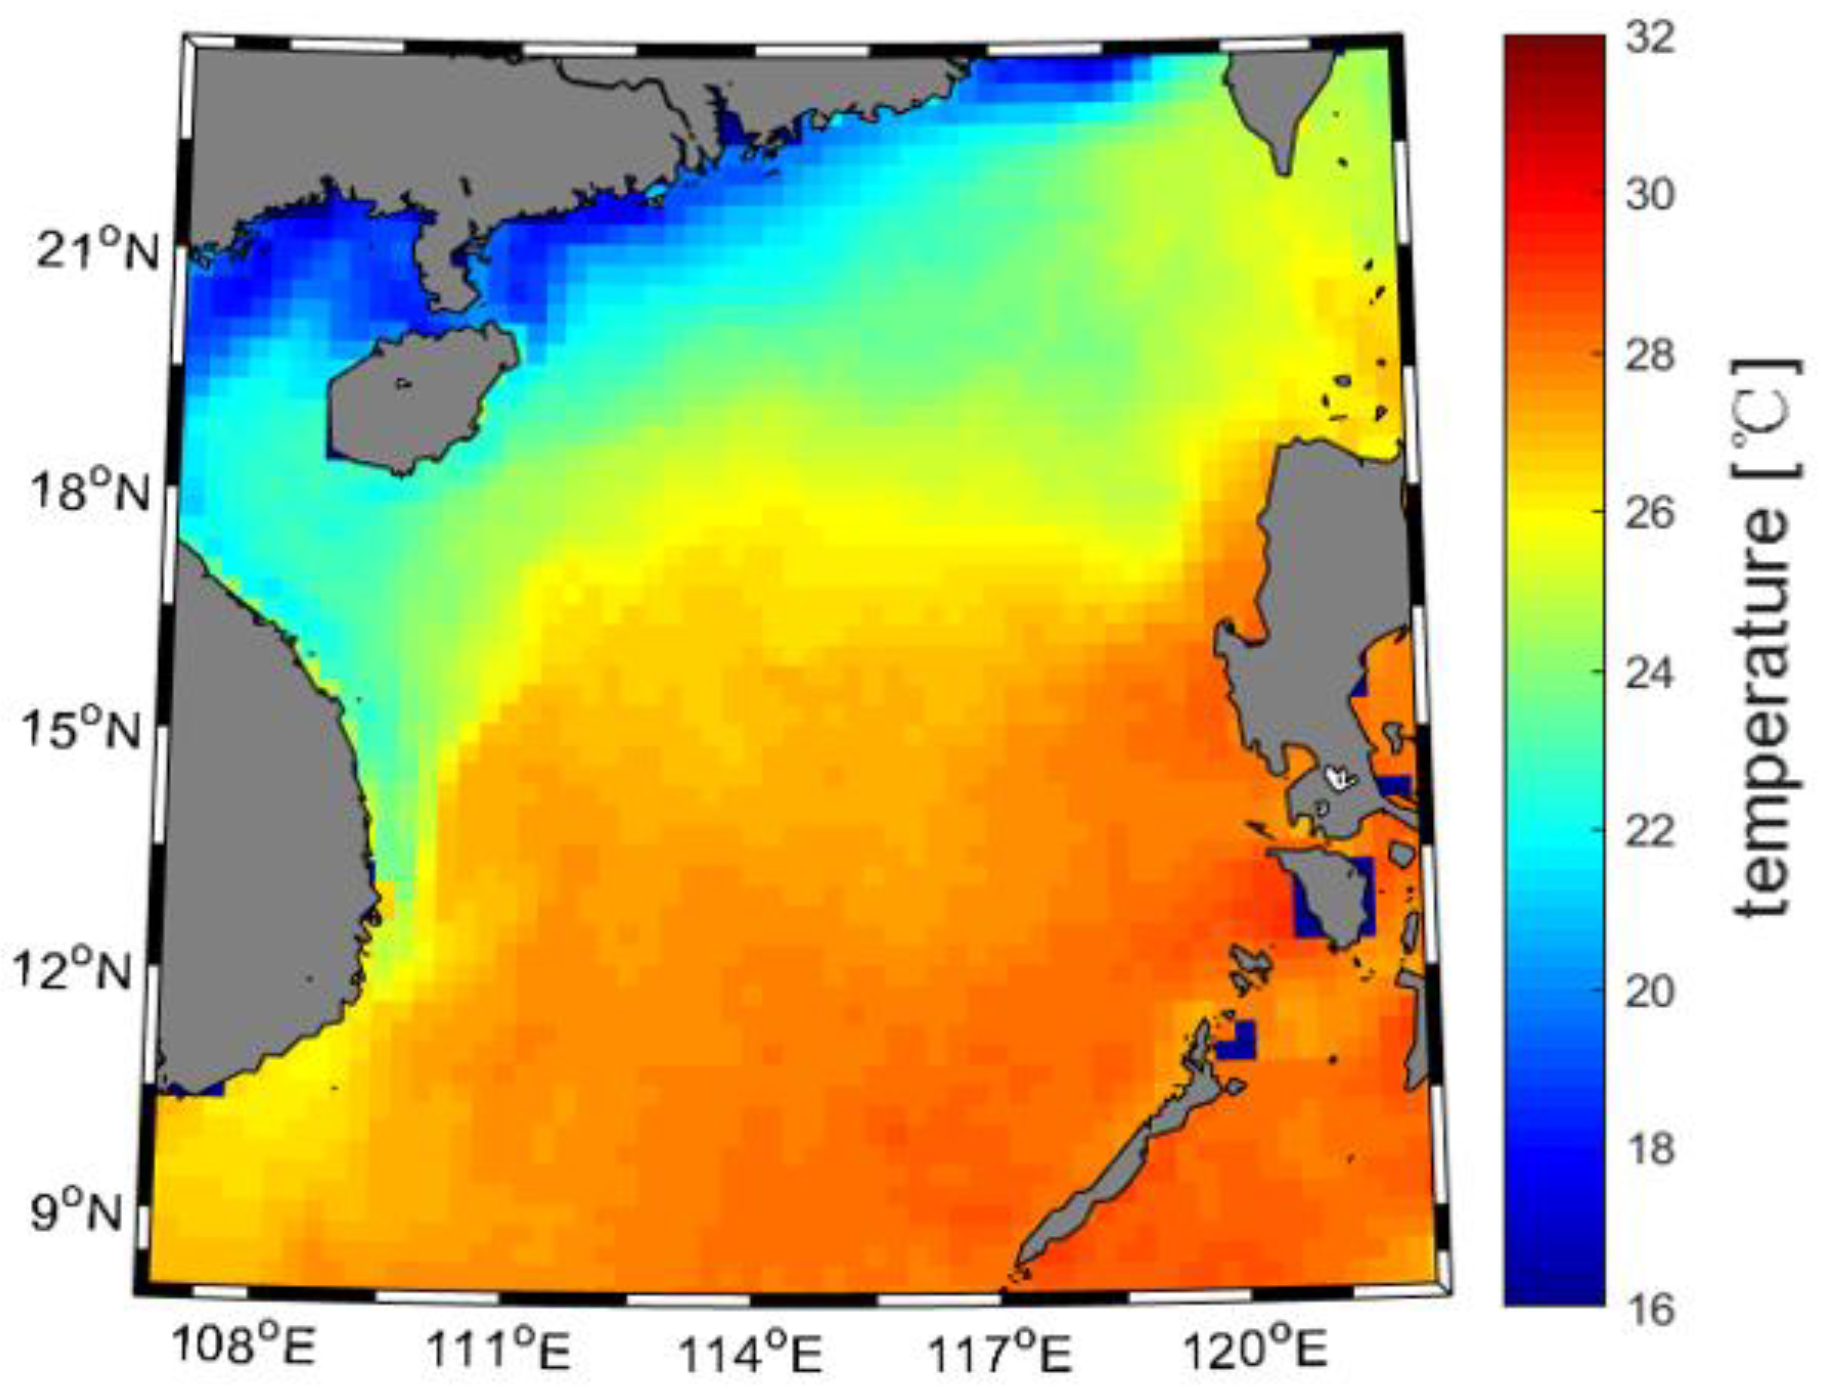
\includegraphics[width=0.9\linewidth]{figures/chapter-1/jmse-11-01030-g001.png}
        \caption{Geospatial data South China sea (Source \cite{jmse11051030})}
        \label{fig:geo-spatial-data-south-china-sea}
    \end{minipage}\hfill
    \begin{minipage}{0.45\textwidth}
        \centering
        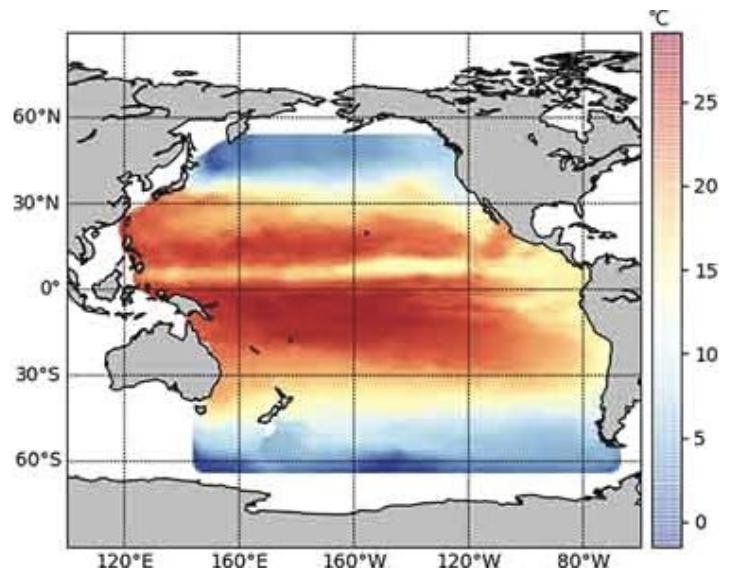
\includegraphics[width=0.9\linewidth]{figures/chapter-1/pacific_ocean.png}
        \caption{Geospatial data Pacific ocean (Source \cite{8913542})}
        \label{fig:geo-spatial-data-pacific-ocean}
    \end{minipage}\hfill
\end{figure}

The above figures shows, that specific areas are considered, South China sea and Pacific Ocean respectively. The data in use is in its primitive form, considering the
latitudes and longitudes of these specific regions. While specific regions are considered, there is still a need for a global representation of the data.

When studying the global phenomenon in climate research, it is essential to take into account the actual characteristics of the surface of the planet. To fully understand
the problems of the global scale, it is essential to accurately depict the global geospatial data on a model that portrays the true nature of the Earth's surface.
Various methodologies have been employed in the literature to address the problem of global representation, and some use different topological surfaces.

One such approach was proposed by Weyn et. al. in 2020 \cite{Weyn_2020}, which involves the utilization of a cubed sphere and consists of six faces generated based on the data
under consideration.
Also, Micha{\"{e}}l Defferrard et. al. in their publication "DeepSphere: a graph-based spherical {CNN}" in 2020 \cite{DBLP:journals/corr/abs-2012-15000} proposed
an architecture named \textbf{DEEPSPHERE}, which is a graph based spherical convolution neural network.

Even though these deep neural network architectures produce results that are on par with the current state-of-the-art models. These architectures still distort the actual
representation of the Earth's surface.
While the issue of accurate representation is still there, these models' heavy usage of GPUs, hardware resources and longer training time begs the question of finding a simpler
model that could represent the global geospatial data and encompass the Earth's surface.

This search of a model which could be used for the representation of the Earth surface motivates us to have a deeper dive in the map projections and their use
in the analysis of the geospatial data on the global scale.
Map projections are the planar projections of the planet Earth, but these planar projections are generated by complex mathematical calculations.
Mainly, map projections are used for the visualization of the geospatial data but their usage for the geospatial data analysis is not conducted thoroughly.


\begin{figure}[h]
    \centering
    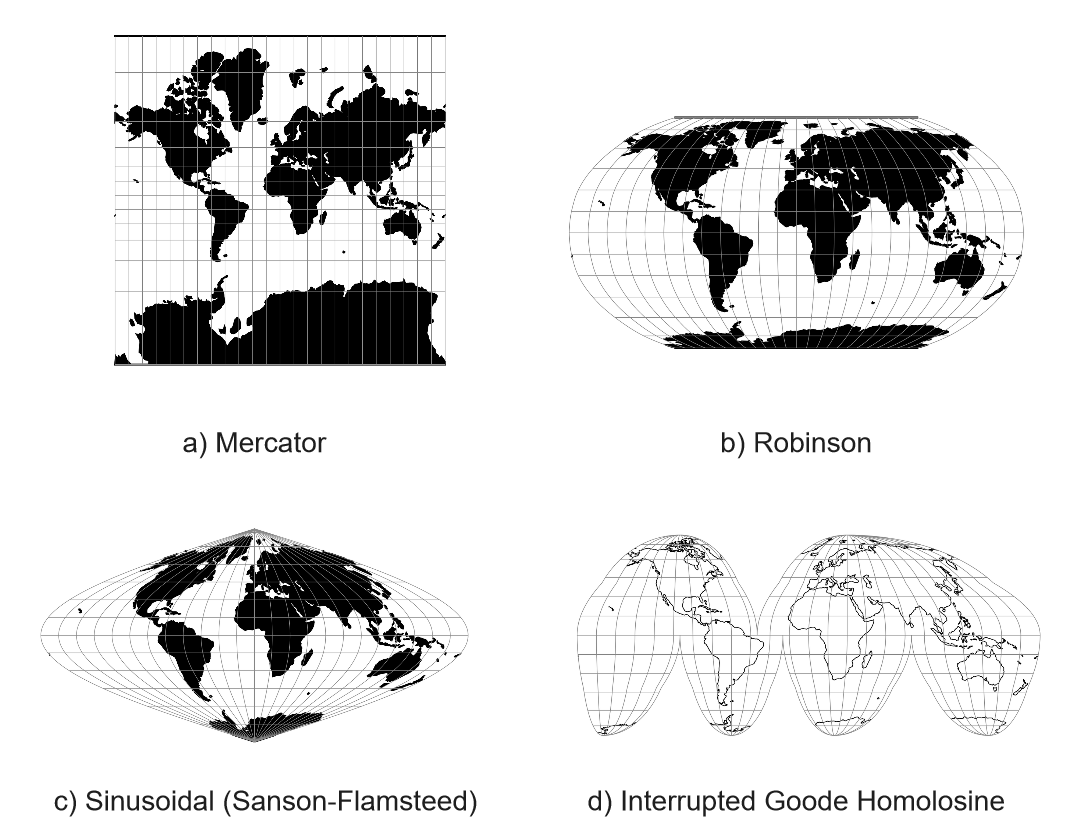
\includegraphics[width=1.0\linewidth]{figures/chapter-1/multi_projections.png}
    \caption{Different map projections (Internal images taken from the source \cite{PROJ_SITE}) }
    \label{fig:multiple-projections}
\end{figure}

Figure \ref{fig:multiple-projections} illustrates four frequently employed projections, yet there exists a plethora of map projections, the selection of which is contingent
upon the particular problem at hand.

Map projections could be a better candidate for the study of the global geospatial data. The planar nature of the map projections are best suited to be studied by the
convolutional neural networks. We can consider a specific map projected geospatial data as a grid, which could be analyzed by the CNNs.
Map projected data could be easily transformed into tensors. This property helps us to use the power of GPUs, making the training process faster. This is the reason
convolutional neural networks (CNNs) are considered for the experimentation.

The thesis is of an exploratory nature which studies the effects of the convolution operation on different map projections. It also provides a framework for verifying
the effects of the convolution operations on different map projection.
The thesis tries to answer the questions, if map projections are used for the geospatial data analysis, from the selected map projections which of them are a better
suited for the task.

\section{Thesis Structure}

This thesis is structured into the chapters outlined as:
\begin{itemize}
    \item \textbf{Chapter 2: (Background Information) } Discusses theoretical background for this study (\autoref{chap:background_information}).
    \item \textbf{Chapter 3: (Related Work) } Discusses existing research in geospatial analysis in global earth system models(\autoref{chap:related_work}).
    \item \textbf{Chapter 4: (Dataset)} Discusses characteristic of geospatial data by global climate simulations (\autoref{chap:dataset}).
    \item \textbf{Chapter 5: (Geo Spatial Data Pre-processing Pipeline)} Focuses on generation of geospatial data rasters  (\autoref{chap:preprocess}).
    \item \textbf{Chapter 6: (Approach)} Dives into the core methodology proposed in thesis.  (\autoref{chap:approach}).
    \item \textbf{Chapter 7: (Experiments and Results)} Showcases the potential of selection for map projection in geospatial analysis  (\autoref{chap:experiments_results}).
    \item \textbf{Chapter 8: (Conclusion and Future Work)} Concludes the research work and suggests future directions for further analysis  (\autoref{chap:conclusion_future_work}).
\end{itemize}
